
This chapter builds the foundation for the thesis introducing relevant concepts and disciplines for the thesis. 


Section \ref{evaluationofmatrix} provides an evaluation of the Matrix security model. The security model is evaluated in the context of a secure messaging system.  
The paper \emph{SoK: Secure Messaging} describes a evaluation framework for evaluating secure messaging systems. They define several security properties related to such systems \cite{sok} which will be presented.


All secure messaging systems with end-to-end encryption are based on the Double Ratchet algorithm from the Signal Protocol which will also be described.


Finally the architecture of Matrix and concepts related to Information-Flow Control will be introduced.

\section{Information security}

Information security is the discipline of protecting information. The key principles in information security are expressed through the CIA model. For a system to be secure these principles should be guaranteed \cite{michael2012}.

\begin{figure}[H]
	\centering
	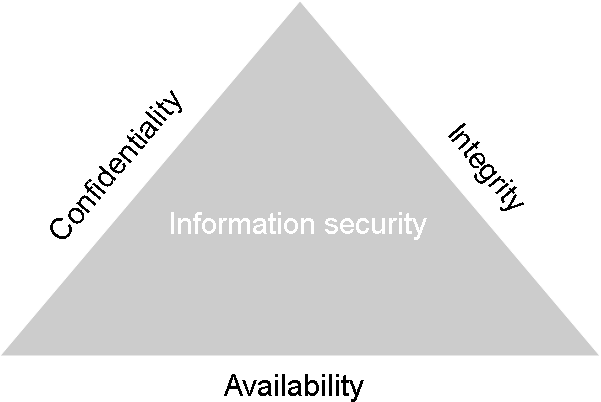
\includegraphics[width=10cm]{figures/cia.png}
	\caption{CIA triad}
	\label{fig:CIA triad}
\end{figure}


\subparagraph{Confidentiality}
Confidentiality is keeping information secret from unauthorized people. This is a major goal in information security. Encryption and access control are common ways of ensuring confidentiality \cite{michael2012}.

In a secure messaging system confidentiality would be guaranteed if the message being sent is only readable by the recipient and no one else \cite{sok}.

\subparagraph{Integrity}
Integrity is providing that information is unaltered and can only be changed by authorized people. If information is intercepted and changed during transit it would be a violation of integrity \cite{michael2012}.  
More specifically for a secure messaging it would mean that no altered message is accepted by the recipient \cite{sok}.

\subparagraph{Availability}
Making sure that information is accessible to authorized people is the goal of availability. Denial of Service attack \footnote{https://en.wikipedia.org/wiki/Denial-of-service\_attack} are common attacks targeting availability. 

Availability is generally more related to the system being available where the information itself plays a minor role \cite{michael2012}.
\\
\\
Depending on the type of system other properties must be satisfied as well. 


\subsection{Security properties}
The goal in a secure messaging system is to protect the messages being sent. The following properties are related to protecting messages.


\subparagraph{Authentication}
When a message is received the participant can verify that the message was sent from the actual sender. Furthermore a participant will receive evidence from a participant in a conversation that hey hold a known long-term secret. 



\subparagraph{Perfect Forward Secrecy}
If all keys are compromised than the decryption of any previously sent message should not be possible. Hence all previous messages would be secure however all future messages would be insecure 

\begin{figure}[H]
	\centering
	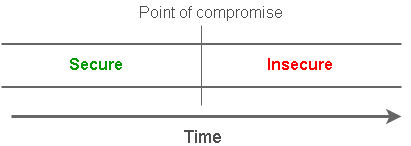
\includegraphics[width=10cm]{figures/forwardsecrecy.png}
	\caption{Forward secrecy}
	\label{fig:forward}
\end{figure}

\subparagraph{Backward secrecy}
If all keys are compromised than the decryption of \emph{future} messages should be possible. This property also goes by the names \emph{future secrecy} and \emph{post compromise security}. 

\begin{figure}[H]
	\centering
	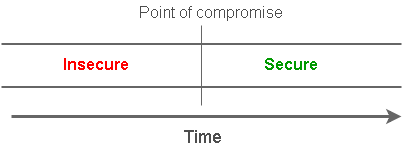
\includegraphics[width=10cm]{figures/backwardsecrecy.png}
	\caption{Backward secrecy}
	\label{fig:backward}
\end{figure}


\subsubsection{Other security properties}


\subparagraph{Participant Consistency} 
Whenever a message is accepted by a participant all participants are guaranteed to have identical view of the participant list.

\subparagraph{Destination Validation}
When a participant receives a message it can be verified that the participant was the intended recipient.

\subparagraph{Anonymity Preserving} 
The anonymity of the participants should be preserved and not linking any key identifiers.

\subparagraph{Speaker Consistency} 
There is consensus among the participants on the sequence of messages they receive by each participant. There might be a mechanism for checking consistency whenever a message is sent or after it has been received.

\subparagraph{Causality Preserving}
Messages must not be displayed before the message that originally precedes it has been displayed.

\subparagraph{Global Transcript} 
A global order where all messages are viewed in the same order for all participants.

\subparagraph{Deniability}
Deniability is a property where other participants cannot confirm that the message being sent was from the sender. Yet during the conversation there will be assurance for the recipient that the message being sent was authentic and sent by the sender \cite{sok}.

\begin{itemize}
	\item \emph{Message Unlinkability:} A deniability property that gives no guarantees that if a participant sent a message that other messages was sent by that participant as well. 
	\item \emph{Message Repudiation:} It can not be proved that a message was authored by a participant given the conversation transcript and all cryptographic key material. 
	\item \emph{Participant Repudiation:} It can not be proved that a participant was in a group conversation without his conversation transcript and cryptographic key material. 
\end{itemize}

The following properties are also defined in the paper \emph{SoK: Secure Messaging} but are less relevant for security.

\subparagraph{Group}

\begin{itemize}
	\item \emph{Computational Equality:} The computational load is equal for all participants.
	\item \emph{Trust Equality:} There is equal trust among all participants. 
	\item \emph{Subgroup messaging:} In the same conversation a participant can send messages to a subset of the participants.
	\item \emph{Contractible Membership:} When a participant leaves a conversation the protocol does not need to restart.
	\item \emph{Expandable Membership:} When a participant joins a conversation the protocol does not need to restart.
\end{itemize}

\subparagraph{Adoption}

\begin{itemize}
	\item \emph{Out-of-Order Resilient:} Messages received out-of-order should be accessible when received.
	\item \emph{Dropped Message Resilient:} On a unreliable network messages might be dropped in transit however it should not prevent decryption of future messages.
	\item \emph{Asynchronous:} Messages can be sent securely to recipients while they are offline.
	\item \emph{Multi-Device Support:} A participant can have multiple devices in a conversation and each device must be synchronized and should have the same historical conversation view
	\item \emph{No Additional Service:} There is no requirement of additional infrastructure being setup other than the participants. 
\end{itemize}





\newpage

\subsection{Concepts}

\subsubsection{Diffie-Hellman Key Exchange}

Diffie-Hellman is a key exchange protocol to establish a shared secret over an insecure channel. Public information is send over an insecure and using asymmetric keys two parties can derive the same shared key.


The first step is to agree on some public values. Either of the parties start the protocol by picking a large prime \emph{p} and a integer \emph{g} then the values are sent over the insecure channel.  

\begin{figure}[H]
	\hspace*{-1cm} 
	\centering
	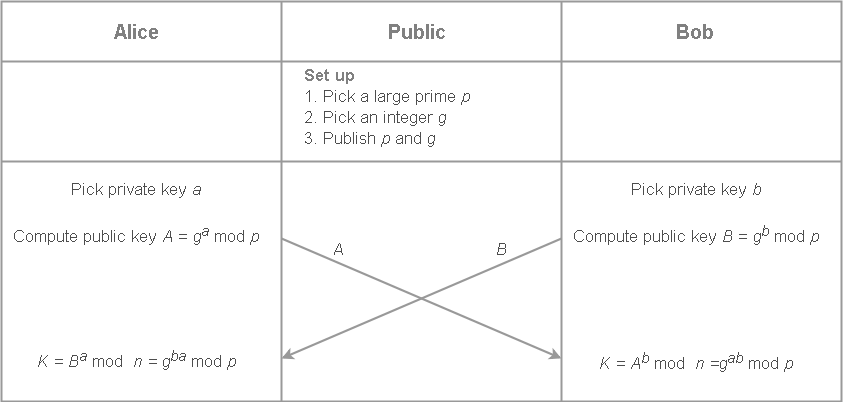
\includegraphics[width=14cm]{figures/dh.png}
	\caption{Simple Diffie-Hellman Key Exchange}
	\label{fig:dh}
\end{figure}

Alice and Bob will each pick a private key value and compute a public key value. The computed key value is sent over the insecure channel and Alice and Bob will both perform the same computation as previously \cite{crypto101}.


The Diffie-Hellman is vulnerable to man in the middle attack since there is no authentication taking place. There exist a solution to this problem using asymmetric key pairs and signing the messages being sent \cite{crypto101}.

\subsubsection{Key Derivation function}

Assume a secret key is established between two parties and is used to encrypt messages and exchange them over an insecure channel. An adversary listening might store all the messages being send even though he is not able to read them. However at some point he manages to compromise the secret key hence being able to decrypting every message ever sent.

To overcome the above scenario ephemeral keys are used. Such keys are short lived and are discarded after use.   

New secret keys can be generated using a \emph{Key Derivation Function} (KDF).
A KDF is a one way function that derives one or more randomized secret keys based on a secret key (or multuple) and optionally some input value \cite{crypto101}. Figure \ref{fig:kdf} illustrates this.

 \begin{figure}[H] 
 	\centering
 	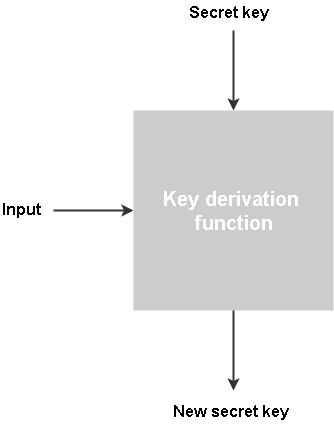
\includegraphics[width=8cm]{figures/kdf.png}
 	\caption{Key derivation function}
 	\label{fig:kdf}
 \end{figure}


A core concept in the Double Ratchet algorithm is KDF chains which build a chain of secret keys using KDF \cite{doubleratchet}. 


\subsubsection{Signal Protocol}

The Signal Protocol provides end-to-end encryption and was developed in 2013 and was first introduced in the app TextSecure\footnote{https://en.wikipedia.org/wiki/TextSecure}.

The Signal Protocol consists of two parts; The \emph{Triple Diffie-Hellman protocol} (TripleDH) and the Double Ratchet algorithm.

\paragraph{Triple Diffie-Hellman protocol}\label{tripledh}
Before the Double Ratchet algorithm can be used the two parties communicating need to agree on a shared secret key. In the Signal protocol this is achieved with Triple Diffie-Hellman protocol \emph{(TripleDH)}.

The Triple Diffie-Hellman protocol is a \emph{key agreement protocol}. It involves a server and two parties; Alice and Bob. 

The TripleDH protocol is characterized by three phases:

\begin{enumerate}
	\item \emph{Publishing keys:} A identity key and several prekeys belonging to Bob is published by him to a server.
	\item \emph{Sending initial message:} Alice sends an initial message to Bob. A prekey bundle is obtained by Alice from the server in order to send an initial message to Bob.
	\item \emph{Receiving initial message:} Alice's message is received and processed by Bob.
\end{enumerate}

\subparagraph{Publishing keys}
Bob needs to register a \emph{prekey bundle} to the server if he wants Alice to be able to send him messages. Alice will likewise have registered a prekey bundle so anyone can to anyone wants to start a message conversation with her.  
The prekey bundle exists of:

\begin{itemize}
	\item Identity key \emph{IK\textsubscript{B}}. This key is only published once by Bob.
	\item Signed prekey \emph{SPK\textsubscript{B}}. This key is reuploaded again after some period of time (eg. after each week or each month). 
	\item Prekey signature \emph{Sig(IK\textsubscript{B}, Encode(SPK\textsubscript{B}))}. This key is also reuploaded again like the signed prekey.
	\item Set of one-time prekeys \emph{(OPK\textsubscript{B}\textsuperscript{1}, OPK\textsubscript{B}\textsuperscript{2}, OPK\textsubscript{B}\textsuperscript{3}, ...)}. These keys are uploaded by Bob occasionally. Bob is informed by the server when there are few one-time prekeys left. 
	
	To ensure forward secrecy the private key of the one-time prekeys are deleted once Bob received messages that uses them. The signed prekey is deleted as well. However Bob might hold on to it for some time to get the messages that was delayed.  
\end{itemize}

\subparagraph{Sending initial message}
Alice retrieves Bobs public keys from the server. She receives one of Bob's single one-time prekey. The server deletes the one-time prekey that was send. It might be the case that all the one-time prekeys at the server has been used \cite{tripledh}.  


Alice verifies the prekey signature if the verification fails the protocol is aborted or else the following public keys are provided to generate a shared secret:

\begin{itemize}
	\item Identity key \emph{IK\textsubscript{A}}. Her own identity key. 
	\item Ephemeral key \emph{EK\textsubscript{A}}. The public key from a generated ephemeral key pair.
\end{itemize}


To generate the shared secret the following calculations are made:

\[DH_1 = DH(IK_A, SPK_B)\]
\[DH_2 = DH(EK_A, IK_B) \]
\[DH_3 = DH(EK_A, SPK_B)\]
\[DH_4 = DH(EK_A, OPK_B)\]
\[SK = KDF(DH_1 || DH_2 || DH_3 || DH_4)\]

There are performed atleast three Diffie-Hellman where \emph{DH\textsubscript{4}} is optional depending on if the server had more one-time prekeys.

Authentication is provided by \emph{DH\textsubscript{1}} and \emph{DH\textsubscript{2}} while \emph{DH\textsubscript{3}} and \emph{DH\textsubscript{4}} provides forward secrecy.

The figure \ref{tripledh} illustrates the calculations. 


\begin{figure}[H]
	\centering
	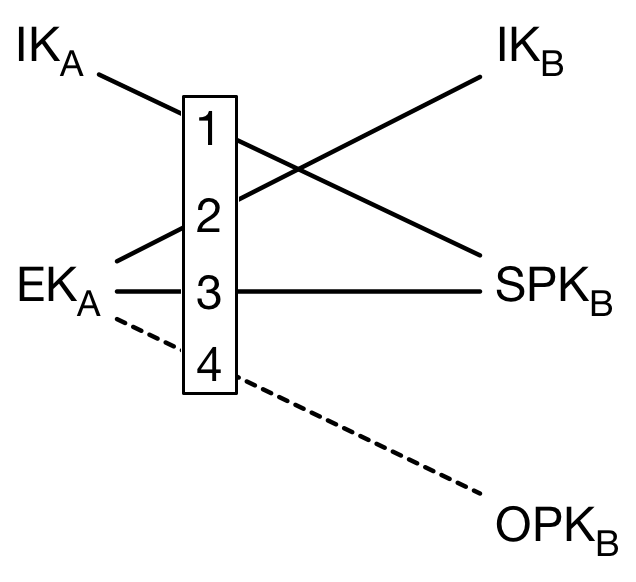
\includegraphics{figures/tripledh.png}
	\caption{Calculations of DH1-DH4 \cite{tripledh}.}
	\label{fig:tripledh}
\end{figure}

Alice then deletes the DH values and her private key associated to the ephemeral key to uphold forward secrecy and sends the initial message to Bob which consists of \cite{tripledh}: 

\begin{itemize}
	\item Cypher text with AEAD encryption  \footnote{https://en.wikipedia.org/wiki/Authenticated\_encryption} with \emph{associated data} using her own and Bob's identity keys.
	\item Her identity key \emph{IK\textsubscript{A}}.
	\item Her ephemeral key \emph{EK\textsubscript{A}}.
	\item Some identifiers to which of Bob's prekeys she used.
	
\end{itemize} 


\subparagraph{Receiving initial message}

When Bob receives Alice's initial message he performs the exact same calculations in phase two and derives the same shared secret key \emph{SK}.

Bob then decrypts the cypher text with the shared key and \emph{associated data} using his own and Alice's identity keys. If the decryption fails the protocol is aborted and \emph{SK} is deleted. Otherwise the protocol is complete and Bob deletes the one-time private prekey. 
The shared secret key can then be used for the Double Ratchet algorithm \cite{tripledh}.  

\paragraph{Double Ratchet algorithm}

After a shared secret key has been established the Double Ratchet algorithm can then be used to send and receive encrypted messages.

Each party has three chains; root chain, sender chain and receive chain. The chains are KDF chains and will take two keys as input (a KDF chain key and some other input key) and output new two keys (a new KDF chain key and some other output key). The KDF chain is illustrated in figure \ref{symkeyratchet}.

The algorithm has a \emph{Diffie-Hellman ratchet} step and \emph{symmetric ratchet} step and the chains are used across both steps.

\begin{itemize}
	\item \emph{Diffie-Hellman ratchet:} The parties exchanges new Diffie-Hellman public keys with the messages being sent. New secrets are then derived using Diffie-Hellman (DH). The secret that DH outputs is used as input to the root chain. The root chain then output new chain keys for the receiving and sending chains. 
	
	\item \emph{Symmetric ratchet:} The sending and receiving chains uses the chain keys derived from the root chain and for each message sent and received the chains are advanced. The output from the receiving and sending chains are keys for encrypting or decrypting messages. 
\end{itemize}


\subparagraph{Symmetric ratchet}
The symmetric ratchet provides message key through the receiving and sending chains. A message key is used for encryption or decryption of a message.

In the symmetric ratchet a single ratchet step is the calculation of the next key chain and message key. The inputs are the current chain key and a constant. Figure \ref{fig:symkeyratchet} illustrates two steps in a symmetric ratchet.

\emph{Forward secrecy} is provided since KDF is a one-way function and it is not possible to go backward and get the input chain key from the output chain key. However since the other input is simply a constant all future keys chain keys and message keys can be derived from an older chain key more specifically there is lack of backward secrecy.


\begin{figure}[H]
	\centering
	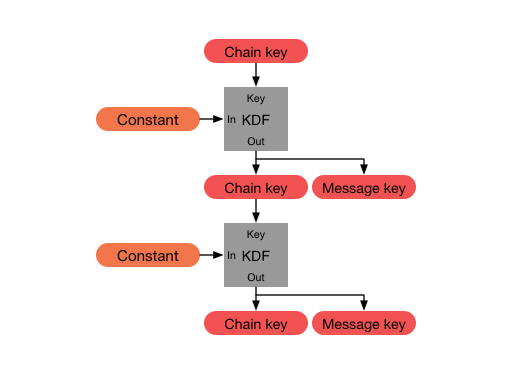
\includegraphics[width=10cm]{figures/symmetrickeyratchet.png}
	\caption{Symmetric key ratchet \cite{doubleratchet}.}
	\label{fig:symkeyratchet}
\end{figure}


\newpage
\subparagraph{Diffie-Hellman ratchet}

Double ratchet provides backward secrecy by comining the Symmetric ratchet with a Diffie-Hellman ratchet hence the name \emph{Double Ratchet}.

Every message from either party begins with a header which contains the sender's current ratchet public key. Whenever a new ratchet public key is received a new ratchet key pair is generated; a secret is derived through Diffie-Hellman with the input being the received ratchet public key and the ratchet private key from the new generated key pair.

Alice starts a conversation with Bob and uses his published public key as a ratchet public key. Alice then generates a new ratchet key pair and derives a shared secret key using Diffie-Hellman and would that as input to her \emph{sending chain}. Alice then sends her new ratchet public key to Bob. At the receiving end Bob derives the same shared secret which would be the input to his \emph{receiving chain}. Alice's sending chain and Bob's receiving chain share the same secret hence he can derive the message key and decrypt the message sent from Alice. When Bob sends a reply to Alice he would generate a new ratchet key pair and derive a new secret which would be input to his \emph{sending chain}.

Figure \ref{fig:dhratchet1} shows an ongoing message exchange with new secrets being derived and the sending and receiving chains being advanced.

\begin{figure}[H]
	\centering
	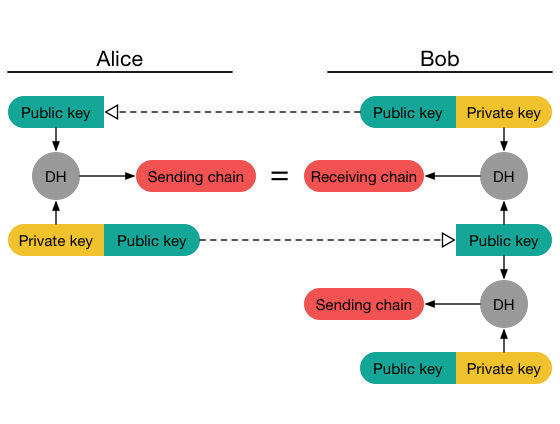
\includegraphics[width=9cm]{figures/dhratchet5.png}
	\caption{Diffie-Hellman ratchet \cite{doubleratchet}.}
	\label{fig:dhratchet1}
\end{figure}


When Alice receive the reply from Bob she would perform the exact same steps. This ultimately results in a continous loop of generating new ratchet key pairs and using Diffie-Hellman to derive the same shared secret key. A continuation is shown in figure \ref{fig:dhratchet2}

\begin{figure}[H]
	\centering
	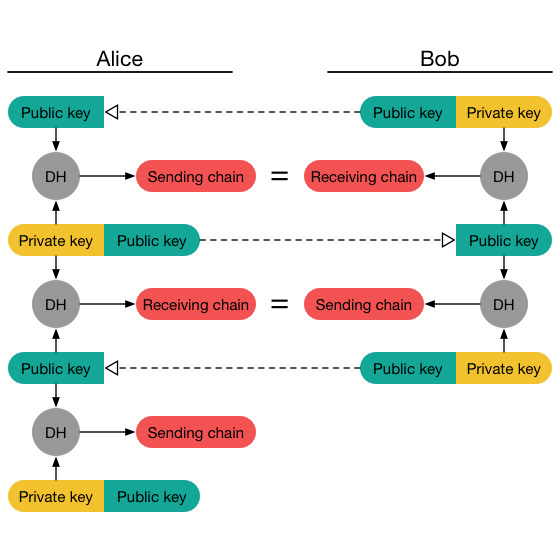
\includegraphics[width=9cm]{figures/dhratchet6.png}
	\caption{Continuation of Diffie-Hellman ratchet  \cite{doubleratchet}.}
	\label{fig:dhratchet2}
\end{figure}


As mentioned in the beginning of the Double Ratchet section the Diffie-Hellman ratchet does have a root chain which would provide inputs to the sending and receiving chains. A more correct view of the process in Diffie-Hellman is shown in figure \ref{fig:dhratchetcon}. 


\begin{figure}[H]
	\centering
	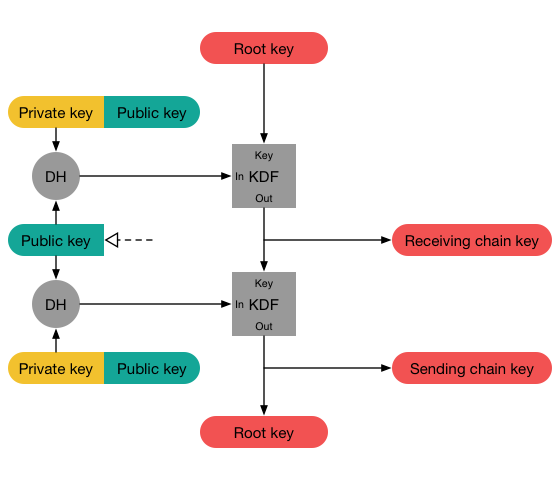
\includegraphics[width=9cm]{figures/dhratchet7.png}
	\caption{Diffie-Hellman ratchet 7 \cite{doubleratchet}.}
	\label{fig:dhratchetcon}
\end{figure}

\paragraph{Double ratchet}

When combining Diffie-Hellman ratchet and symmetric-key ratchet the result is the Double ratchet.

\begin{itemize}
	\item When sending or receiving a message the corresponding message key is derived by performing a symmetric-key ratchet step.
	\item Upon receiving a new ratchet public key the Diffie-Hellman ratchet step performed right before the symmetric-key ratchet step with the goal of replacing old chain keys with new ones.  
\end{itemize}

Assume that the message exchanged is a continuation from the TripleDH key exchange described in section \ref{tripledh}. Alice had sent an initial message. The initial ratchet public key would be Bob's signed prekey \emph{SPK\textsubscript{B}} and the new ratchet key pair would be the Alice's ephemeral key pair that she generated. Alice calculated a shared secret which is the \emph{root key}. She then generates a new ratchet key pair and takes the output from Diffie-Hellman and use it as input for the \emph{root chain}. The root chain then outputs a new root key \emph{RK} and a sending chain key {CK}.

The figure \ref{doubleratchet1} depicts this with a view of Alice's chains.


\begin{figure}[H]
	\centering
	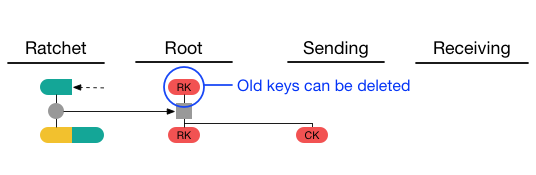
\includegraphics[width=10cm]{figures/doubleratchet1.png}
	\caption{Double ratchet 1 \cite{doubleratchet}.}
	\label{fig:doubleratchet1}
\end{figure}

When Alice then sends a message \emph{A1} the symmetric-key ratchet step will return a new chain key and a message key. The message can then be encrypted with the message key.

\begin{figure}[H]
	\centering
	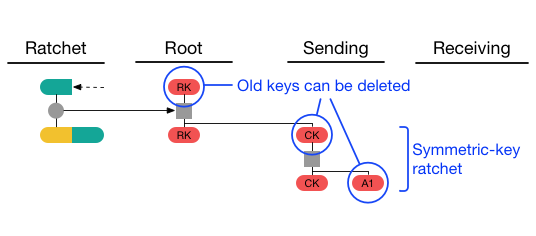
\includegraphics[width=10cm]{figures/doubleratchet2.png}
	\caption{Double ratchet 2 \cite{doubleratchet}.}
	\label{fig:doubleratchet2}
\end{figure}

Next Alice receives a message \emph{B1} from Bob. The message header contains a new ratchet public key and a Diffie-Hellman ratchet step is performed. New sending and receiving chain keys are derived and followed by a symmetric-key ratchet step to derive the receiving message key to decrypt the message.

\begin{figure}[H]
	\centering
	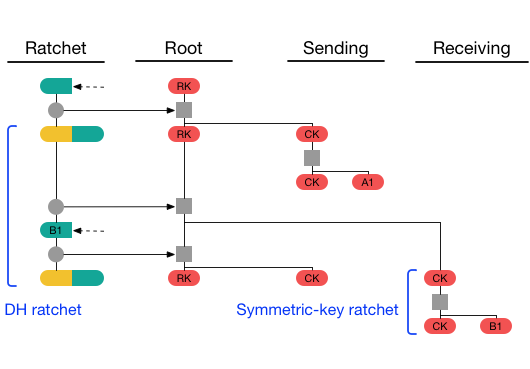
\includegraphics[width=10cm]{figures/doubleratchet3.png}
	\caption{Double ratchet 3 \cite{doubleratchet}.}
	\label{fig:doubleratchet3}
\end{figure}





\newpage
\section{Matrix}

\subsection{Goals}

\subsubsection{Short term goal}

\subsubsection{Long term goal}
% https://www.youtube.com/watch?v=-ofZMnKkp_Y 5:00 , 18:30

\subsection{How does it work?}

\subsection{Architecture}

\subsection{Matrix specification}

\subsection{End-to-end Encryption}





\newpage
\section{Information Flow Control} %mere konkret og teknisk
%Selvom jeg ikke kiggr på fx trafic analysis så er det vigtigt at nævne og påpege det ikkeer noget jeg løser

\subsection{The Lattice Model}
adsadsad

\subsection{Noninterference}
dasdsa

\subsection{Static policies}


sadsad
\subsection{Dynamic policies}
sadsadsad


\subsection{Declassification}
Taking some specific information and changing it to a lower security classification.

Identify: What to classify, who declassifies, where the declassification happens and when the declassification happens

\section{Summary}
